%!TEX program = xelatex
\documentclass[a4paper,UTF8]{ctexart}

\usepackage{fontspec}
\usepackage{amsmath}
\usepackage{float}
\usepackage{graphicx}
\usepackage{amssymb}
\usepackage{epstopdf}
\usepackage{mathrsfs}
\usepackage{stmaryrd}
\usepackage{color}
\usepackage{listings}
\usepackage{ulem}
\usepackage{lmodern}
\usepackage[margin=2cm]{geometry}
\usepackage{titlesec}
\usepackage{svg}
\usepackage{tikz}
\usepackage{hyperref}
\usepackage[noblocks]{authblk}
\usepackage{MyTitle}

% 对于使用 Texpad 打开本 TeX 文档的用户,请使用这行代码
\usepackage[cache=false,outputdir=.texpadtmp]{minted}
% 其它用户使用这行
%\usepackage{minted}
%

\setlength{\parskip}{5pt}

\titleformat{\section}[hang]{\bfseries\fontsize{16pt}{0pt}\selectfont}{\thesection}{.5em}{}{}


%To do: 修改标题和作者及联系方式
\title{HITCON2015 Quals, Crypto100, Simple}

\author{邓雄飞(DeathKing)}
\affil{哈尔滨工业大学,计算机科学与技术学院,dk@hit.edu.cn}

\date{}

\begin{document}
\maketitle

\begin{center}
\parbox{0.9\textwidth}{
\textbf{摘~~~要}\quad 本文是 HITCON2015 Quals 比赛 Simple 一题的题解,主要介绍了此题的解题思路和解题方法。同时,本文探讨了在使用AES-128-CFB加密模式下,攻击者如何利用泄露的初始化向量(Initial Vector),巧妙地构造恶意密文并使服务器还原为我们想要的原文的方法。\\
\textbf{关键词}\quad HITCON, CTF, Crypto, Ruby, AES, CFB, Cookies Attack\\}
\end{center}


%------------------------------------------------------------------------------------------------------------------------------
%------------------------------------------------------------------------------------------------------------------------------
%To do: 正文开始
%------------------------------------------------------------------------------------------------------------------------------
%------------------------------------------------------------------------------------------------------------------------------

\section{题目描述}

本题是密码学范畴一道分值为 100 的题目,其描述如下:\\

\begin{quizdesc}[label=Crypto100 Simple]
Become admin!

http://52.69.244.164:51913
simple-01018f60e497b8180d6c92237e2b3a67.rb
\end{quizdesc}

题干中只告知选手“成为管理员”,并提供了一个端口供选手进行攻击。该端口上运行着一个 Ruby 脚本,这是一个 Sinatra 应用,其具体代码如下:

%\linespread{1}
\begin{minted}{ruby}
#!/usr/bin/env ruby

require 'sinatra/base'
require 'sinatra/cookies'
require 'openssl'
require 'json'

KEY = IO.binread('super-secret-key')
FLAG = IO.read('/home/simple/flag').strip

class SimpleApp < Sinatra::Base
  helpers Sinatra::Cookies

  get '/' do
    auth = cookies[:auth]
    if auth
      begin
        auth = auth.b
        c = OpenSSL::Cipher.new('AES-128-CFB')
        c.decrypt
        c.key = KEY
        c.iv = auth[0...16]
        json = c.update(auth[16..-1]) + c.final
        r = JSON.parse(json)
        if r['admin'] == true
          "You're admin! The flag is #{FLAG}"
        else
          "Hi #{r['username']}, try to get admin?"
        end
      rescue StandardError
        'Something wrong QQ'
      end
    else
      <<-EOS
<html><body><form action='/' method='POST'>
<input type='text' name='username'/>
<input type='password' name='password'/>
<button type='submit'>register!</button>
</form></body></html>
      EOS
    end
  end

  post '/' do
    username = params['username']
    password = params['password']
    if username && password
      data = {
        username: username,
        password: password,
        db: 'hitcon-ctf'
      }
      c = OpenSSL::Cipher.new('AES-128-CFB')
      c.encrypt
      c.key = KEY
      iv = c.random_iv
      json = JSON.dump(data)
      enc = c.update(json) + c.final
      cookies[:auth] = iv + enc
      redirect to('/')
    else
      'Invalid input!'
    end
  end
end
\end{minted}

\section{解题思路}

\subsection{程序运行流程}\label{program-workflow}

通过阅读提供的源码文件,我们发现这是一个非常简单的 Web 应用,以至于该应用只有\code{get '/'}和\code{post '/'}两个路由。

\code{get '/'} 路由的执行效果会因 Cookie 中是否含有 \code{auth} 一项而不同。如果 Cookie 中不含 \code{auth} 一项,那么系统会显示一张含有 \code{username} 和 \code{password} 项的表单,要求用户填写并提交此表单。如果 Cookie 中含有 \code{auth} 一项,那么服务器会将该项 Cookie 的前 16 个字节作为初始化向量,配合在服务器中存储的密钥 \code{KEY} 对 Cookie 后面的内容进行解密,并将解密的内容视为 JSON 字符串解析。如果解析出的 JSON 对象包含 \code{admin} 属性且值为 \code{true} ,则会向客户端回复包含 FLAG 的字符串,否则提示错误信息。在 Cookie 解密和 JSON 解析的过程中,出现任何异常都会被 \code{rescue StandError} 子句捕获到。这样,有用的错误信息会被可以隐藏,选手只能得到 \code{"Something wrong QQ"} 的提示。

\code{post '/'} 路由用于处理提交的表单。为了防止选手故意构造 \code{POST} 表单,直接在表单中注入类似于 \code{admin: true} 等信息,脚本在编写时,显式地指明了只使用 \code{username}  和 \code{password} 属性。服务端会将利用这两个属性构造的 \code{data} 散列序列化为一个 JSON 字符串 \code{`json`},并在 AES-128-CFB 模式下进行加密。加密用到的初始化向量是随机生成的,使用到的密钥 \code{KEY} 存放在服务器中。需要注意的是,在最后生成的 Cookie 中,前16个字节是加密过程中使用的初始化向量,后面的字节才是加密后的 JSON 字符串。

根据题目和源码分析的情况来看,我们需要想方设法“成为管理员”,这样就可以得到本题的 FLAG 我们不难想到本题应该在 Cookie 上做文章。一种思路就是:精心构造 Cookie ,使得服务端解密还原该 Cookie 后,会得到一个含有 \code{'admin': true} 项的 JSON 字串。这样,在服务器反序列化此 JSON 字符串后,我们即可得到管理员权限。

\subsection{漏洞分析}

直观地来说,如果我们能知道系统采用的加密方案(使用到的算法、相关密钥的选择等),那么我们就能合理地构造出符合我们要求的密文。但是,由于加密用的密钥 \code{KEY} 是存放在服务器上的,如果不使用渗透范畴的技术,那么这个密钥应被视为“不可取得的”,我们需要思考其它的方法。

为了分析整个系统的漏洞,我们需要审视一下 AES-128-CFB 加密方案的工作流程\cite{wiki_aes}\cite{wiki_bcmo}。需要说明的是 AES-128-CFB 是一种加密方案,它的各项指标解释如下:

\begin{enumerate}
  \item AES:高级加密标准(Advanced Encryption Standard),是一种对称密钥加密的区块加密标准,其具体实现为比利时密码学家 Joan Daemen 和 Vincent Rijmen 所设计 Rijndael 加密法。AES 的密文块长度固定为 128 位。
  \item 128:密钥长度为 128 位,即 16 字节。
  \item CFB:密文反馈(Cipher feedback),这是一种块密码的工作模式,它使得我们能够使用同一个块密码密钥对多于一块的数据进行加密,并保证其安全性。在CFB工作模式下,前一个区块加密(解密)出的密文,将用于后一个区块的加密(解密)过程中。
\end{enumerate}

\begin{figure}[hbt!]
  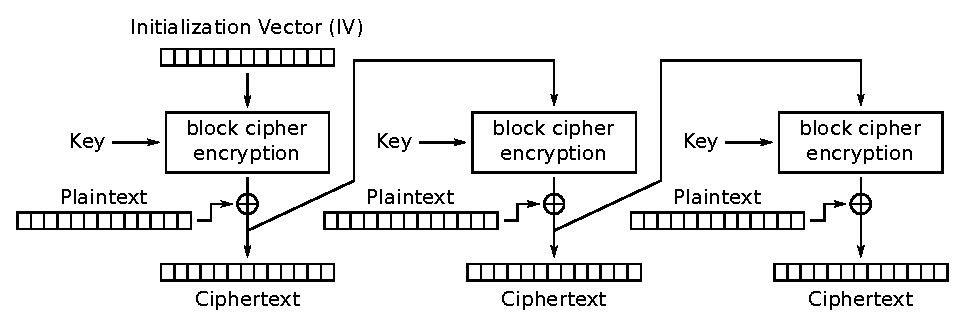
\includegraphics{CFB_encryption.eps}
  \caption{CFB 加密模式}\label{cfb-enc}
\end{figure}

图 \ref{cfb-enc} 介绍的是该方案的加密过程。首先,将明文划分为数个128位的块 $P_i$,对于第一个区块来说,首先运行 AES 加密函数加密 $E_{K}(\mathrm{IV})$ , 其中,$K$ 是秘密选择的密钥, $\mathrm{IV}$ 是初始向量。然后,将算得的结果与明文块 $P_0$ 进行异或运算,得到第一个密文块 $C_0$ 。并将 $C_0$ 当作下一区块的初始向量,重复此过程,直到所有明文都被加密。该过程可以描述为下面的公式:

\begin{eqnarray}
  C_i & = & E_K(C_{i-1}) \oplus P_i \\
  P_i & = & E_k(C_{i-1}) \oplus C_i \\
  C_0 & = & \mathrm{IV}
\end{eqnarray}

\begin{figure}[hbt!]
  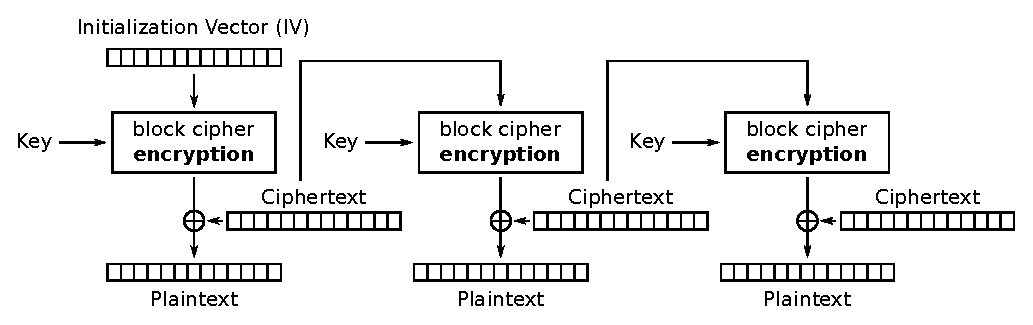
\includegraphics{CFB_decryption.eps}
  \caption{CFB 解密模式}\label{cfb-dec}
\end{figure}

图 \ref{cfb-dec} 介绍的是该方案的加密过程。对应地,首先需要将密文划分为数个128位的块 $C_i$ 。与其它工作模式不同,CFB工作模式下使用加密过程中的加密函数来对密文解密,不需要额外的解密函数。解密过程使用与加密过程相同的初始向量 $\mathrm{IV}$ 和密钥 $K$ 。密文块 $C_i$ 将被用作下一个区块的初始化向量进行解密。重复此过程,直到所有明文都被解密。该过程可以描述为下面的公式:

\begin{eqnarray}
  P_i & = & E_k(C_{i-1}) \oplus C_i \\
  C_{-1} & = & \mathrm{IV}
\end{eqnarray}

仔细观察加密、解密公式,由于我们无法获知加密使用的密钥 \code{KEY} ,且密文会作为反馈,作用于下一个区块。因此,我们不能轻易地根据明文构造任意长度的密文。如果仔细观察源码,服务器只会检查 \code{admin} 一项的属性,考虑到 JSON 字符串 \code{{'admin':true}} 只有 14 个字符,即 14 字节。因此在一个密码区块内考虑此问题是足够的,此时,将 $i=0$ 分别带入加密、解密方程组,不难得到下面的等式:

\begin{eqnarray}
  P_0 \oplus C_0 & = & E_K(\mathrm{IV}) \label{important}
\end{eqnarray}

显然,$E_K(\mathrm{IV})$ 是个常量。如果我们能得到这个常量的值,并控制等式中另外一个量,那么,剩余的那个量也就可以被我们间接控制了。我们的攻击,就基于这个等式。

\section{解题过程}
 
\subsection{第一步:获得 $E_K(\mathrm{IV})$}

考虑式 \ref{important} ,在我们的攻击中,$P_0$ 是由我们输入的,$C_0$ 可以从服务器返回的 Cookie 中取得,因此这两个量都是已知量,因此可以由此计算出 $E_K(\mathrm{IV})$ 。

\subsection{第二步:构造 $C_0^\prime$}

继续考虑式 \ref{important} ,为了让服务器解密得到原文 $P_0^\prime = \text{\{'admin':true\}}$ ,我们可以将式 \ref{important} 做移项变换得到构造公式 $ C_0^\prime = P_0^\prime \oplus E_K(\mathrm{IV})$ ,这样我们就可以算得构造出来的密文了。

\subsection{第三步:篡改 Cookie}

利用第二步构造出来的密文,篡改服务器生成的 Cookie ,再次触发 \code{get '/'} 路由,即可看到 FLAG。

\subsection{使用到的脚本}

下面这段 Ruby 脚本可用于辅助构造密文,需要将 \code{construct} 变量设定为我们想要服务器还原的原文,将 \code{strcookie} 设定为从服务器获得的 Cookie ,我们需要以 \code{1} 作为 \code{username} 提交HTML表单。脚本中使用到了 \code{rack} 库,其中提供的 \code{escape} 和 \code{unescape} 方法可用于 Cookie 的转义与反转义。


%\begin{minted}[linenos,
%               %numbersep=5pt,
%               %gobble=2,
%               xleftmargin=.1\textwidth,
%  			   xrightmargin=.1\textwidth,
%               framerule=0.8pt,
%               frame=lines,
%               framesep=2mm]{ruby}
\begin{minted}{ruby}
#!/usr/bin/env ruby

require 'rack'

# Ya, Monkey patching.
class Array
  def xor(ary)
    raise RuntimeError, "Size doesn't match." unless size == ary.size
    self.zip(ary).map{ |a, b| a^b }
  end
end

# The first 128bit block we input:
plain     = '{"username":"1",'
# The plaintext we want the server decode to:
construct = '{"admin":true  }'
# The cookie we get from the server:
strcookie = 'THE-COOKIE'

cookie = Rack::Utils.unescape(strcookie)

iv = cookie.bytes[0..15]
c0 = cookie.bytes[16..31]

# Calculate the E_K(IV)
ekiv = c0.xor plain.bytes

# Construct the ciphertext
c0_prime = ekiv.xor construct.bytes

# This is the result
cookie = (iv + c0_prime).map(&:chr).join
puts Rack::Utils.escape(cookie)

\end{minted}

%\section{参考文献}

%\small

\begin{thebibliography}{99}
\setlength{\parskip}{0pt}  %段落之间的竖直距离

\bibitem{wiki_aes} Advanced Encryption Standard, \url{https://en.wikipedia.org/wiki/Advanced_Encryption_Standard}
\bibitem{wiki_bcmo} Block cipher mode of operation, \url{https://en.wikipedia.org/wiki/Block_cipher_mode_of_operation}
\bibitem{sch07} Schneier B. Applied cryptography: protocols, algorithms, and source code in C[M]. john wiley \& sons, 2007.
\end{thebibliography}


%------------------------------------------------------------------------------------------------------------------------------
%OK: 正文结束
%------------------------------------------------------------------------------------------------------------------------------


\end{document}
